\subsubsection{Motivation}
A cut-based top jet tagger is applied in 2015 paper for this analysis\cite{CMS-PAS-SUS-16-030}. The cut-based top jet tagger has a wonderful efficiency over the top pt spectrum. However, the mistag rate is also relatively high in this tagger. Therefore, we design a new top tagger to reduce the mistag rate. 

\subsubsection{Description of the method}
\label{sec:toptagger}

Before we move to the top tagger algorithm, let’s review the top decay modes. The top jet decay (Fig~\ref{fig:c4twdecaymod}) can be categorized into two classes: hadronically decayed tops and leptonically (and semi-leptonically) decayed tops. We focus on the hadronically decayed tops since we are searching SUSY in hadronic channels. The hadronically decayed tops can majorly be detected in three ways (Fig~\ref{fig:c4twdecaymod}): a fat mono-jet with mass close to top mass, a fat mono-jet with mass close to W mass and one b-jet, and 3 resolved jets. Our cut-based algorithm is designed following these three scenarios respectively. 

\begin{figure}[htbp]
 \begin{center}
  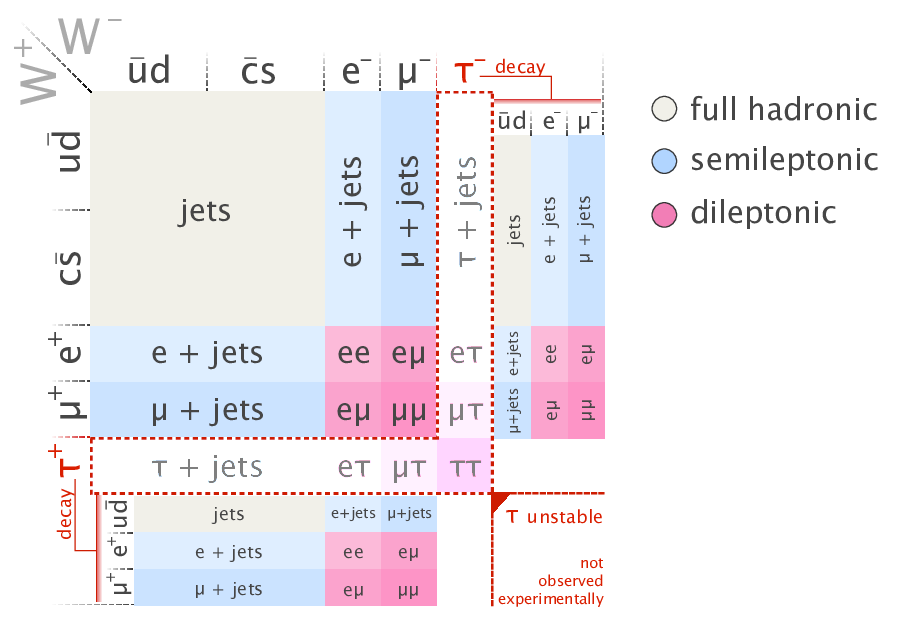
\includegraphics[width=0.55\textwidth]{figures/c4/c4_top_w_decaymod.png}
  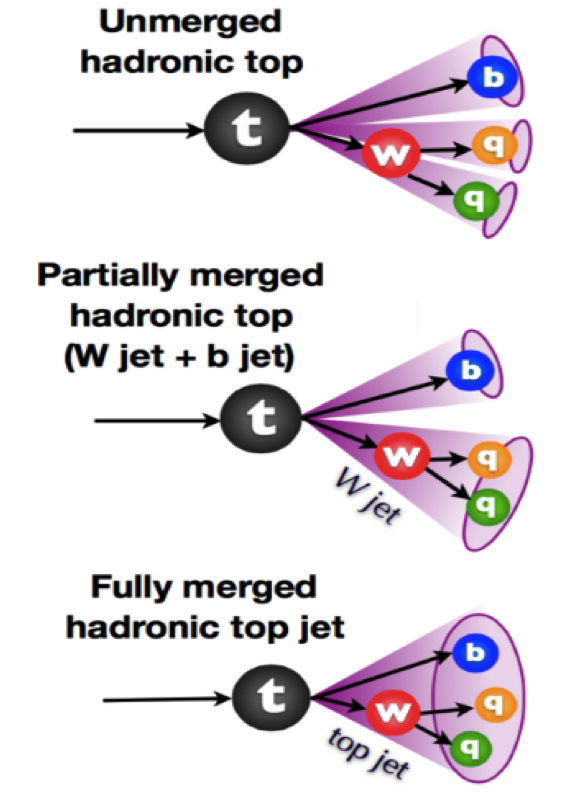
\includegraphics[width=0.25\textwidth]{figures/c4/c4_tagger_hadtopdecay.png}
 \end{center}
 \caption{Left: \ttbar events final states; Right: Hadronically decayed tops}
 \label{fig:c4twdecaymod}
\end{figure}

Only the small AK4 cone jet collection is used in the cut-based tagger to avoid jet removing from different collections. The side effect of this treatment is the remnant system can be relatively big in the mono-jet and di-jet case. The cut-based algorithm is not very powerful in the tri-jets system, compared with multi-variable algorithms. Therefore, the new top tagger has 2 major upgrades: fat jet (AK8 jet) for mono-jet and di-jet top decay, and multi-variable algorithm for tri-jet system. We expect lower mistag rate with the similar efficiencies after the upgrade. 

The mono-jet top selection is relatively simple. The requirements for the mono-AK8 jet are:
\begin{itemize}
\item AK8 jet $p_{T}\ge$400 GeV 
\item Soft drop mass between 105 and 210 GeV
\item N-subjettiness $\tau_{32}\le$0.65
\end{itemize}

If an AK8 jet is used in the mono-jet case, it will be removed from the jet collection for next steps. 

We require one W-like AK8 jet and b-like AK4 jet in the di-jet case. The W-like AK8 jet is selected with following requirements:
\begin{itemize}
\item AK8 jet $p_{T}\ge$200 GeV
\item Soft drop mass between 65 and 100 GeV
\item N-subjettiness $\tau_{21}\le$0.60
\end{itemize}

Then, the W-like AK8 jet will be combined with one AK4 jet with $p_{T}\ge$40 GeV. The additional requiremnets on the di-jet system is:
\begin{itemize}
\item di-jet system mass is between 100 to 250 GeV
\item di-jet system within R cone 1.0
\item jet mass ratio between AK8 W-like jet and di-jet system in range $[ 0.85 \frac{m_{W}}{m_{t}}, 1.25 \frac{m_{W}}{m_{t}} ]$
\end{itemize}

We start using both AK4 and AK8 jet collections from this step. We design an overlap remove algorithm to avoid jet energy reusing in the algorithm. A $\Delta R$ matching between AK4 jets and soft-drop sub-jets of the AK8 jets is applied for jet removal. 

As we mentioned before, multi-variable algorithm is applied to select the tri-jets top. There are two key elements in the multi-variable algorithm design: input variables and algorithm. 

In general, we have two input variables types: the high-level physics variables, like jet $p_{T}$, and base level physics variable, like particle flow candidate, and calorimeter pixels. The algorithm choosing is dependent on the input variables. For example, the high-level variables are more suited for the decision tree based algorithm, while base level variables prefer neutral network. 

We choose the high-level physics variables and decision tree based algorithm in our analysis. All three-jets combinations will be the potential top candidates. The following variables are considered in the algorithm: 
\begin{itemize}
\item Top candidate properties: mass, $p_{T}$, R cone size;
\item Constituent jet properties: jet $p_{T}$, $\eta$, $\phi$; CSV value (b-tag likelyhood), quark-gluon discriminator;
\item Angular variables between jets: $\Delta \phi, \Delta \eta, \Delta R$
\end{itemize}
%todo add QGL

All the variables are carefully studied before we put them into training. Let’s use quark gluon discriminator as an example. The quark gluon discriminator is likelihood to separate the quark jet and gluon jet. The value of the likelihood close to 1 means it is more like a quark jet, otherwise a gluon jet. The likelihood is constructed from three variables: 
\begin{itemize}
\item $p_{T}$D: jet energy dispersion variable, defined as $ $, with sum over all PF candidates
\item Mutiplicity: the total number of particle flow candidates that reconstructed within the jet
\item Axis2: minor axis RMS in the $\eta - \phi$ plane of the particle flow candidates
\end{itemize}

The multi-variable algorithm is better in digging out the correlation between training variables. The algorithm with the clean input variables can obtain the correlation features. Therefore, we need to study the performance of quark gluon discriminator on different jet flavors, $p_{T}$ and $\eta$. We studied the following jet flavors in the ttbar simulation samples: light flavor jet, c-jet, b-jet, gluon jet and pile-up jet. The $p_{T}$ and $\eta$ schemes are listed in the Table~\ref{tab:c4ttqgl}.

\begin{table}[htbp]
\fontsize{10 pt}{1.2 em}
\selectfont
\begin{centering}
\caption{\label{tab:c4ttqgl} Jet bin for quark-gluon discriminator study}
\hspace*{-4ex}
\begin{tabular}{|c|c|c|c|c|c|c|}
\hline
Jet $\eta$ Bin  & 1(HB) & 2(HBHE) & 3(HE) & 4(HEHF) & 5(HF) & 6(HF,no PDF) \\
\hline
Jet $\eta$      & [0,1.305] & [1.305,1.392] & [1.392,2.650] & [2.650,3.139] & [3.139,4.7] & [4.7,5.191] \\
\hline
Jet $p_{T}$ Bin & 1(no PDF) & 2 & 3 & 4 & 5 & 6 \\
\hline
Jet $p_{T}$     & [0,20] & [20,40] & [40,50] & [50,80] & [80,100] & [100,Inf] \\
\hline
\end{tabular}
\par\end{centering}
\end{table}

The performance in terms of jet $\eta$ in different jet flavors is showed in Fig~\ref{fig:c4ttqgljeteta}. The discrimination power for low $p_{T}$ jets is not ideal. 
\begin{figure}[htbp]
 \begin{center}
  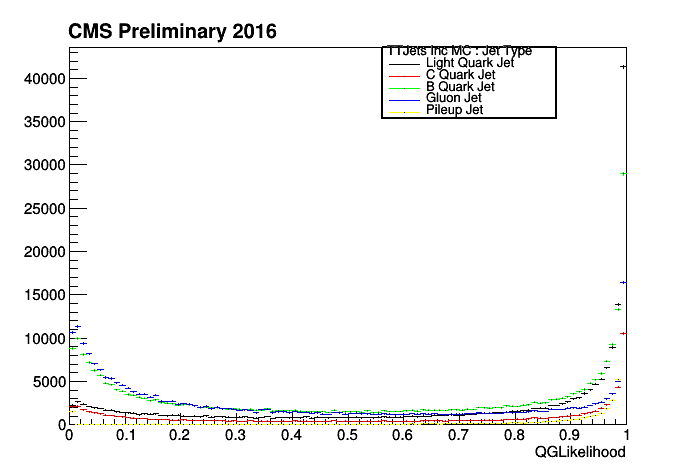
\includegraphics[width=0.45\textwidth]{sections/mc4/TopTagger/figures/_b_qglikelihoodjetetabin0_.png}
  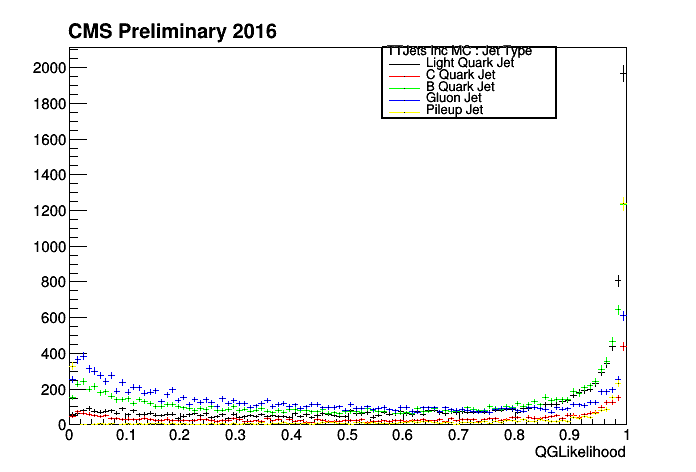
\includegraphics[width=0.45\textwidth]{sections/mc4/TopTagger/figures/_b_qglikelihoodjetetabin1_.png} \\
  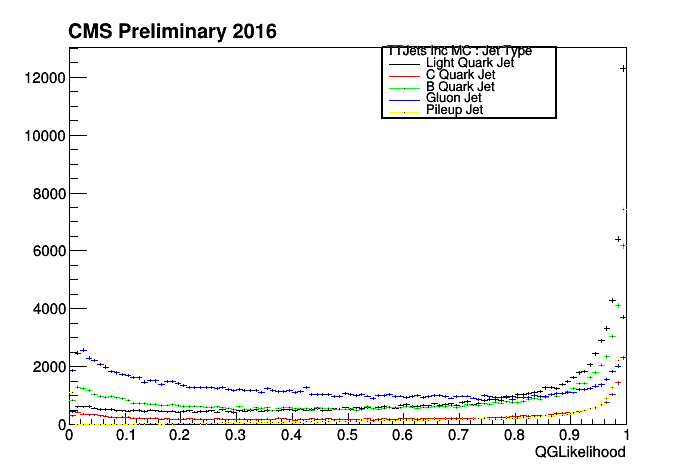
\includegraphics[width=0.45\textwidth]{sections/mc4/TopTagger/figures/_b_qglikelihoodjetetabin2_.png}
  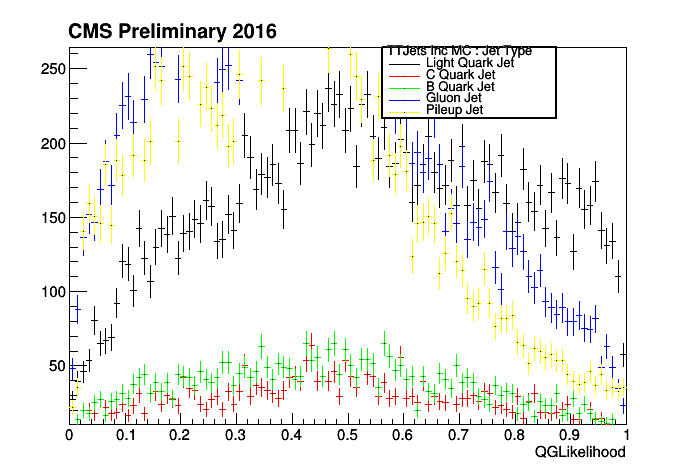
\includegraphics[width=0.45\textwidth]{sections/mc4/TopTagger/figures/_b_qglikelihoodjetetabin3_.png} \\
  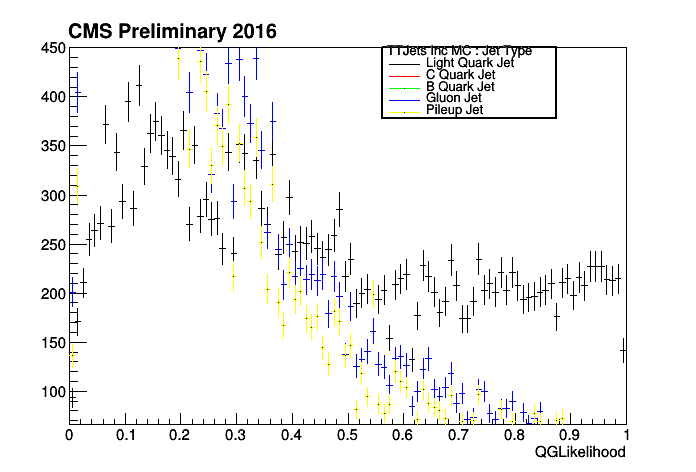
\includegraphics[width=0.45\textwidth]{sections/mc4/TopTagger/figures/_b_qglikelihoodjetetabin4_.png}
  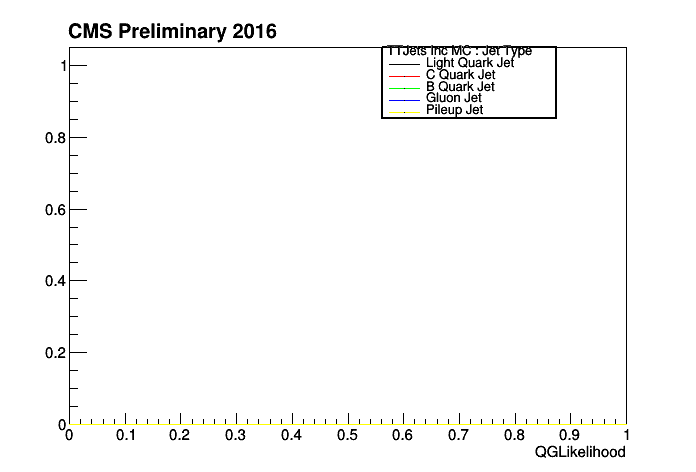
\includegraphics[width=0.45\textwidth]{sections/mc4/TopTagger/figures/_b_qglikelihoodjetetabin5_.png}
 \end{center}
 \caption{Top left: Quark Gluon likelihood for jet $\eta$ bin 1; Top right: jet $\eta$ bin 2; Middle left: jet $\eta$ bin 3; Middle right: jet $\eta$ bin 4; Middle left: jet $\eta$ bin 5; Middle right: jet $\eta$ bin 6}
 \label{fig:c4ttqgljeteta}
\end{figure}

The performance in terms of jet $p_{T}$ in different jet flavors is showed in Fig~\ref{fig:c4ttqgljetpt}. The discrimination power for HEHF and HF jets is not ideal.
\begin{figure}[htbp]
 \begin{center}
  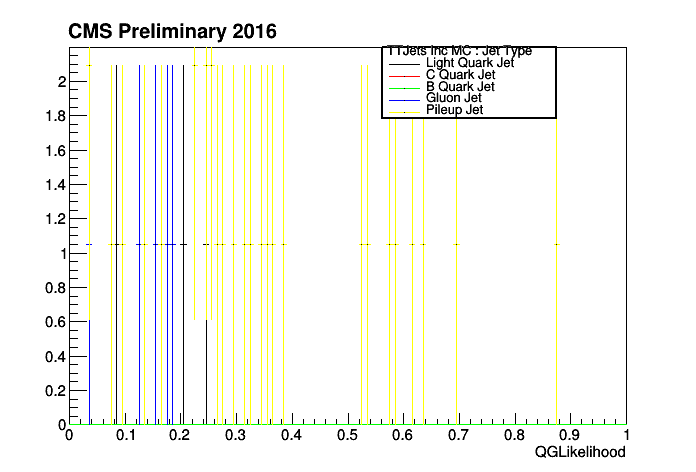
\includegraphics[width=0.45\textwidth]{sections/mc4/TopTagger/figures/_b_qglikelihoodjetptbin0_.png}
  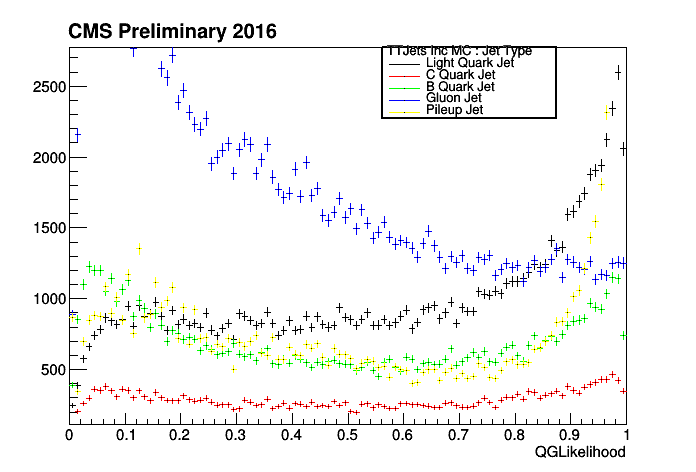
\includegraphics[width=0.45\textwidth]{sections/mc4/TopTagger/figures/_b_qglikelihoodjetptbin1_.png} \\
  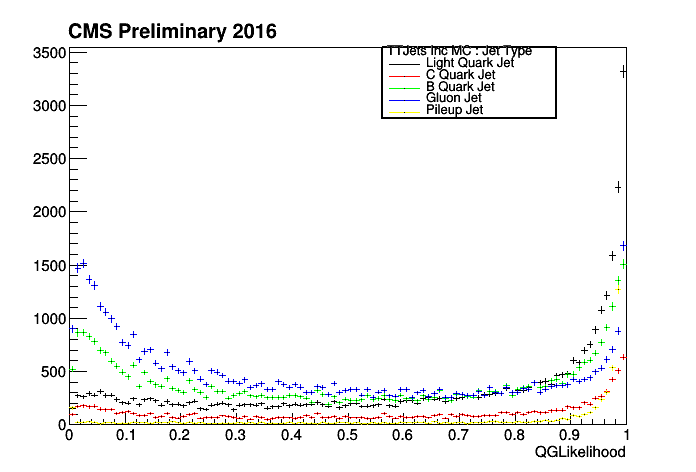
\includegraphics[width=0.45\textwidth]{sections/mc4/TopTagger/figures/_b_qglikelihoodjetptbin2_.png} 
  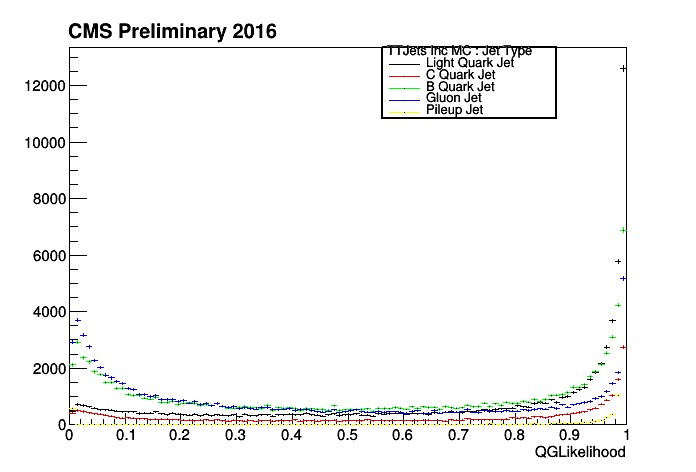
\includegraphics[width=0.45\textwidth]{sections/mc4/TopTagger/figures/_b_qglikelihoodjetptbin3_.png} \\
  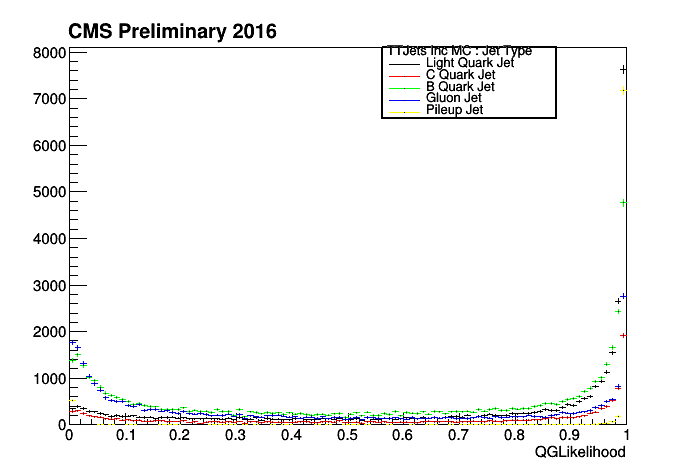
\includegraphics[width=0.45\textwidth]{sections/mc4/TopTagger/figures/_b_qglikelihoodjetptbin4_.png}
  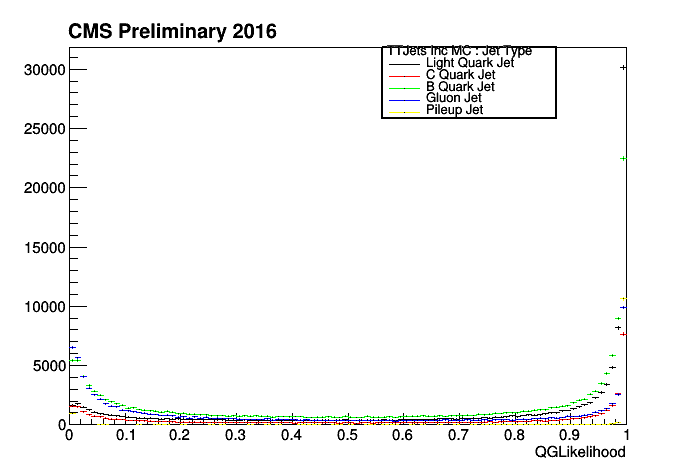
\includegraphics[width=0.45\textwidth]{sections/mc4/TopTagger/figures/_b_qglikelihoodjetptbin5_.png}
 \end{center}
 \caption{Top left: Quark Gluon likelihood for jet $p_{T}$ bin 1; Top right: jet $p_{T}$ bin 2; Middle left: jet $p_{T}$ bin 3; Middle right: jet $p_{T}$ bin 4; Middle left: jet $p_{T}$ bin 5; Middle right: jet $p_{T}$ bin 6}
 \label{fig:c4ttqgljetpt}
\end{figure}

And, the quark gluon discriminator is now working well with b-jet for all cases. Therefore, we decide to force the likelihood to be 1 (quark jet) in case of a tagged b-jet before training. 

All the variables are feed into random forest\cite{Ho:1995:RDF:844379.844681} training algorithm for training in simulation samples. We designed three working points in different efficiencies-mistag rate balance. Finally we choose the tight working points for the search after sensitivity study. The combined top-jet reconstruction efficiencies (Fig~\ref{fig:c4ttefftight}) are about 0.6. The mistag rate (Fig~\ref{fig:c4ttmistagtight}) about 0.2, 50\% reduced compared with the cut-based legacy tagger. Now, we complete our tagging algorithm in full simulation samples. We still need to study the difference between the full simulation and data, and also full simulation and fast simulation, since we are using fast simulation signals for limit setting. The scale factors are binned in the top-jet $p_{T}$ and applied in the data card before limit setting. More details are demonstrated in\cite{AN-16-461}. 

\begin{figure}[htbp]
 \begin{center}
  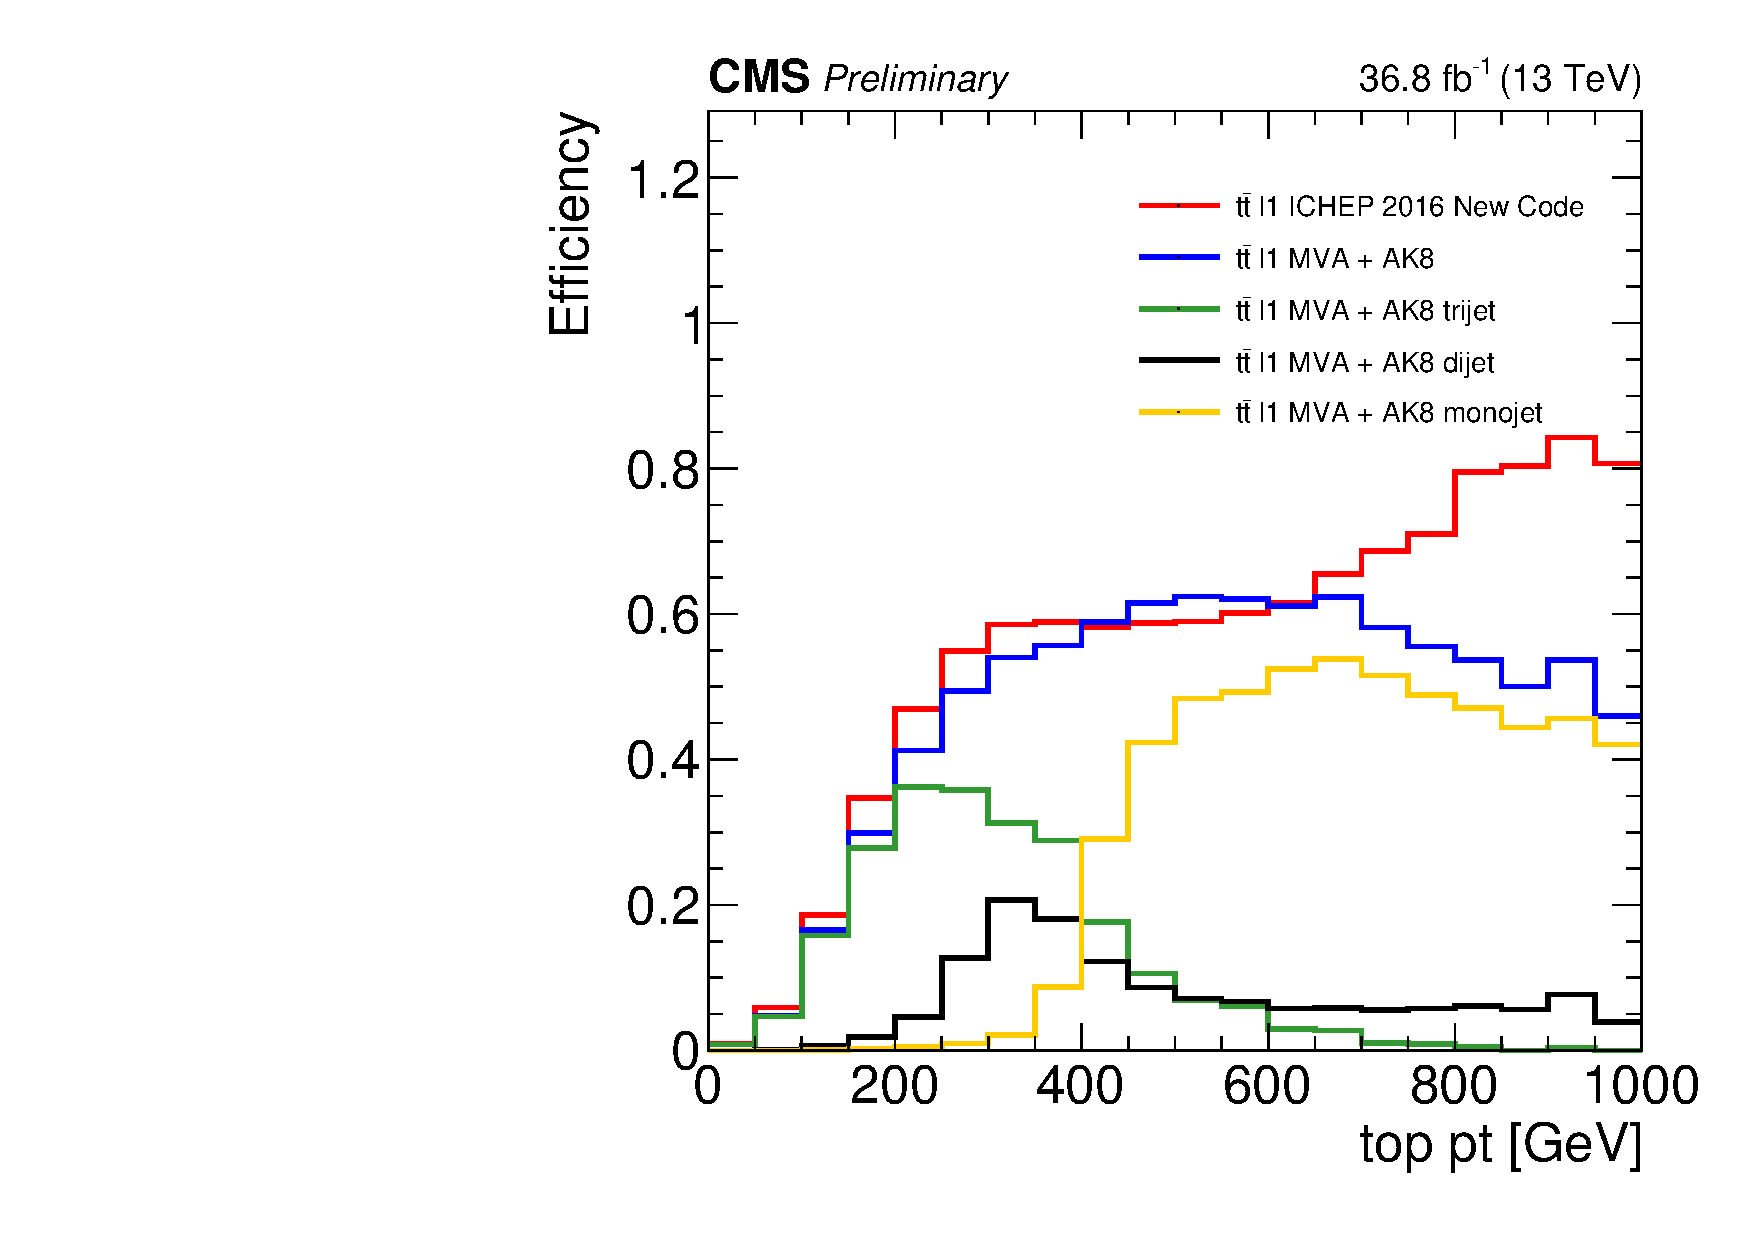
\includegraphics[width=0.85\textwidth]{sections/mc4/TopTagger/figures/baseline_eff_pt_ttbar1l_tight.pdf}
 \end{center}
 \caption{Top-jet reconstruction efficiencies, measured in \ttbar simulation samples}
 \label{fig:c4ttefftight}
\end{figure}

\begin{figure}[htbp]
 \begin{center}
  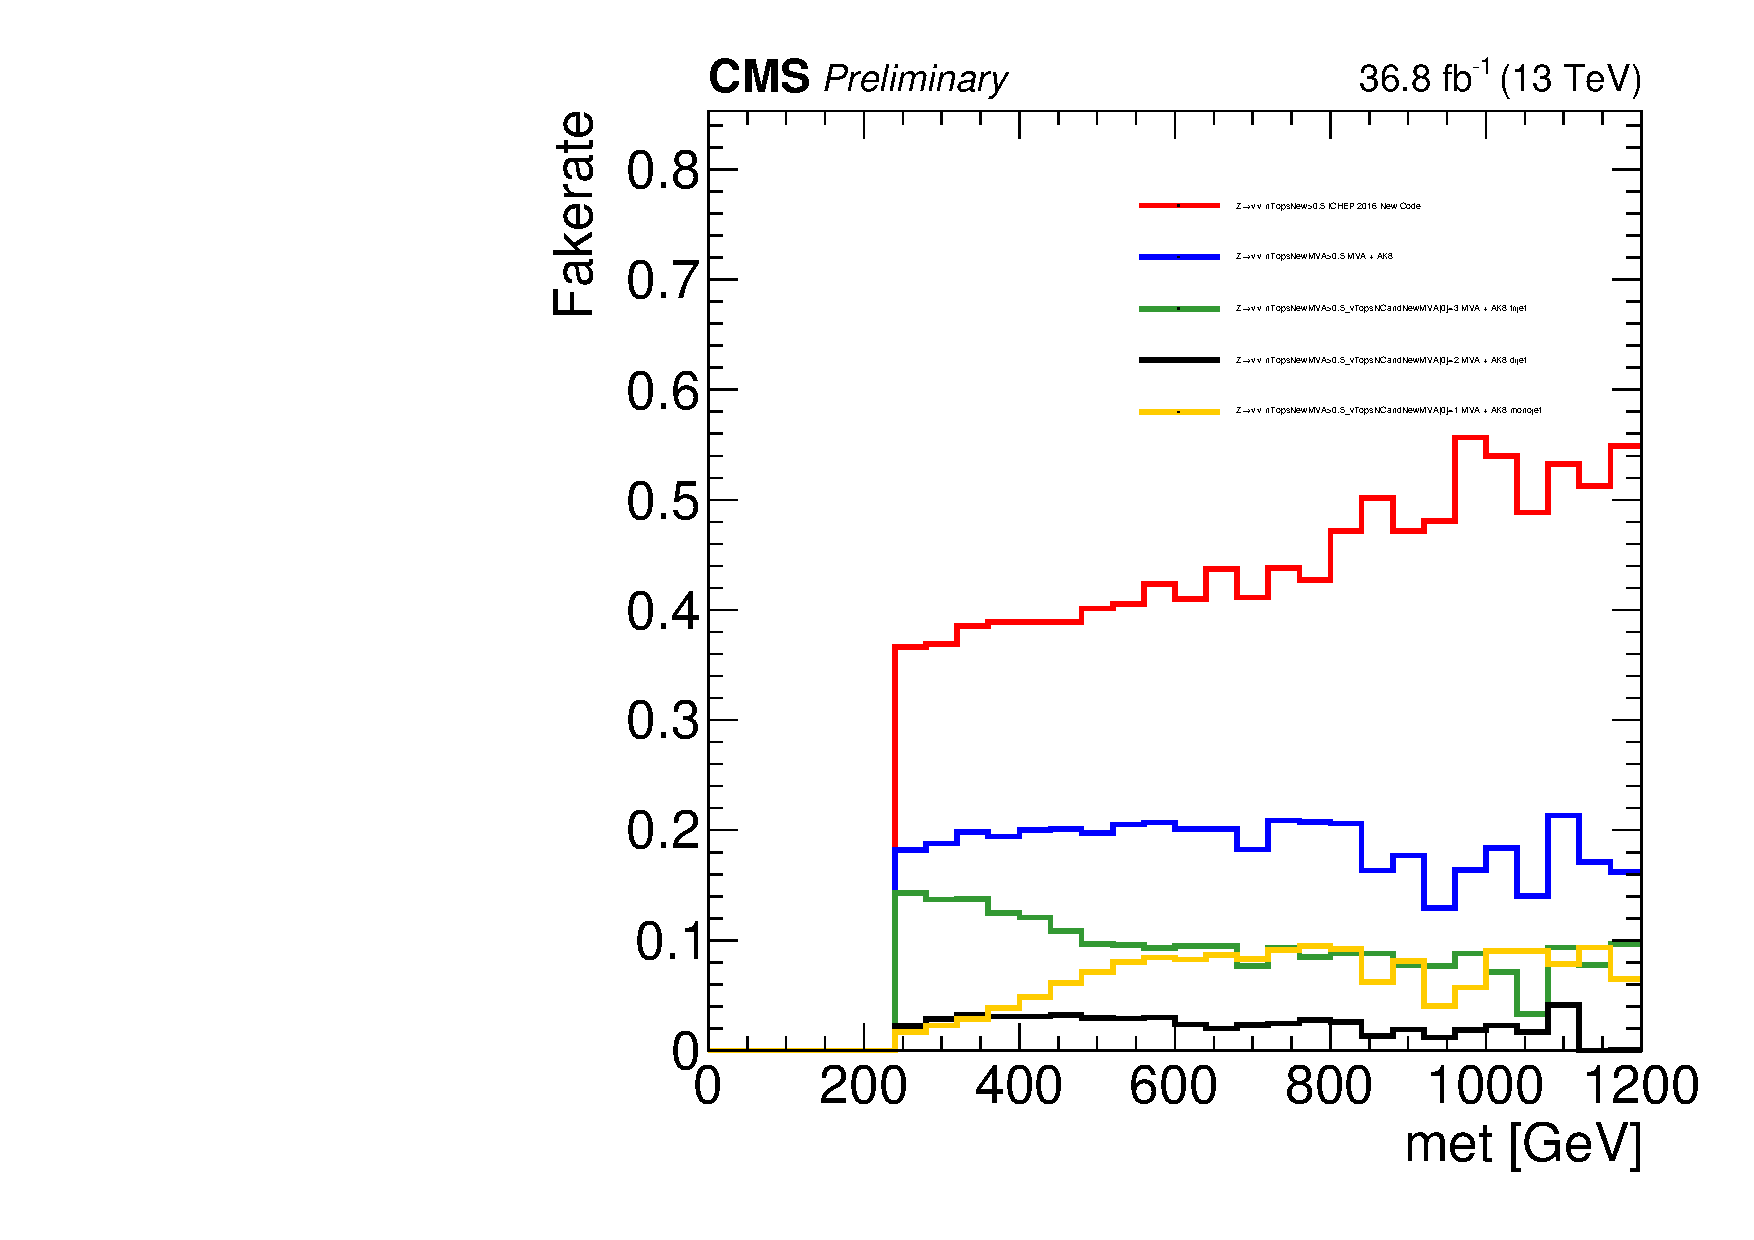
\includegraphics[width=0.45\textwidth]{sections/mc4/TopTagger/figures/baseline_fakerate_met_tight.pdf}
  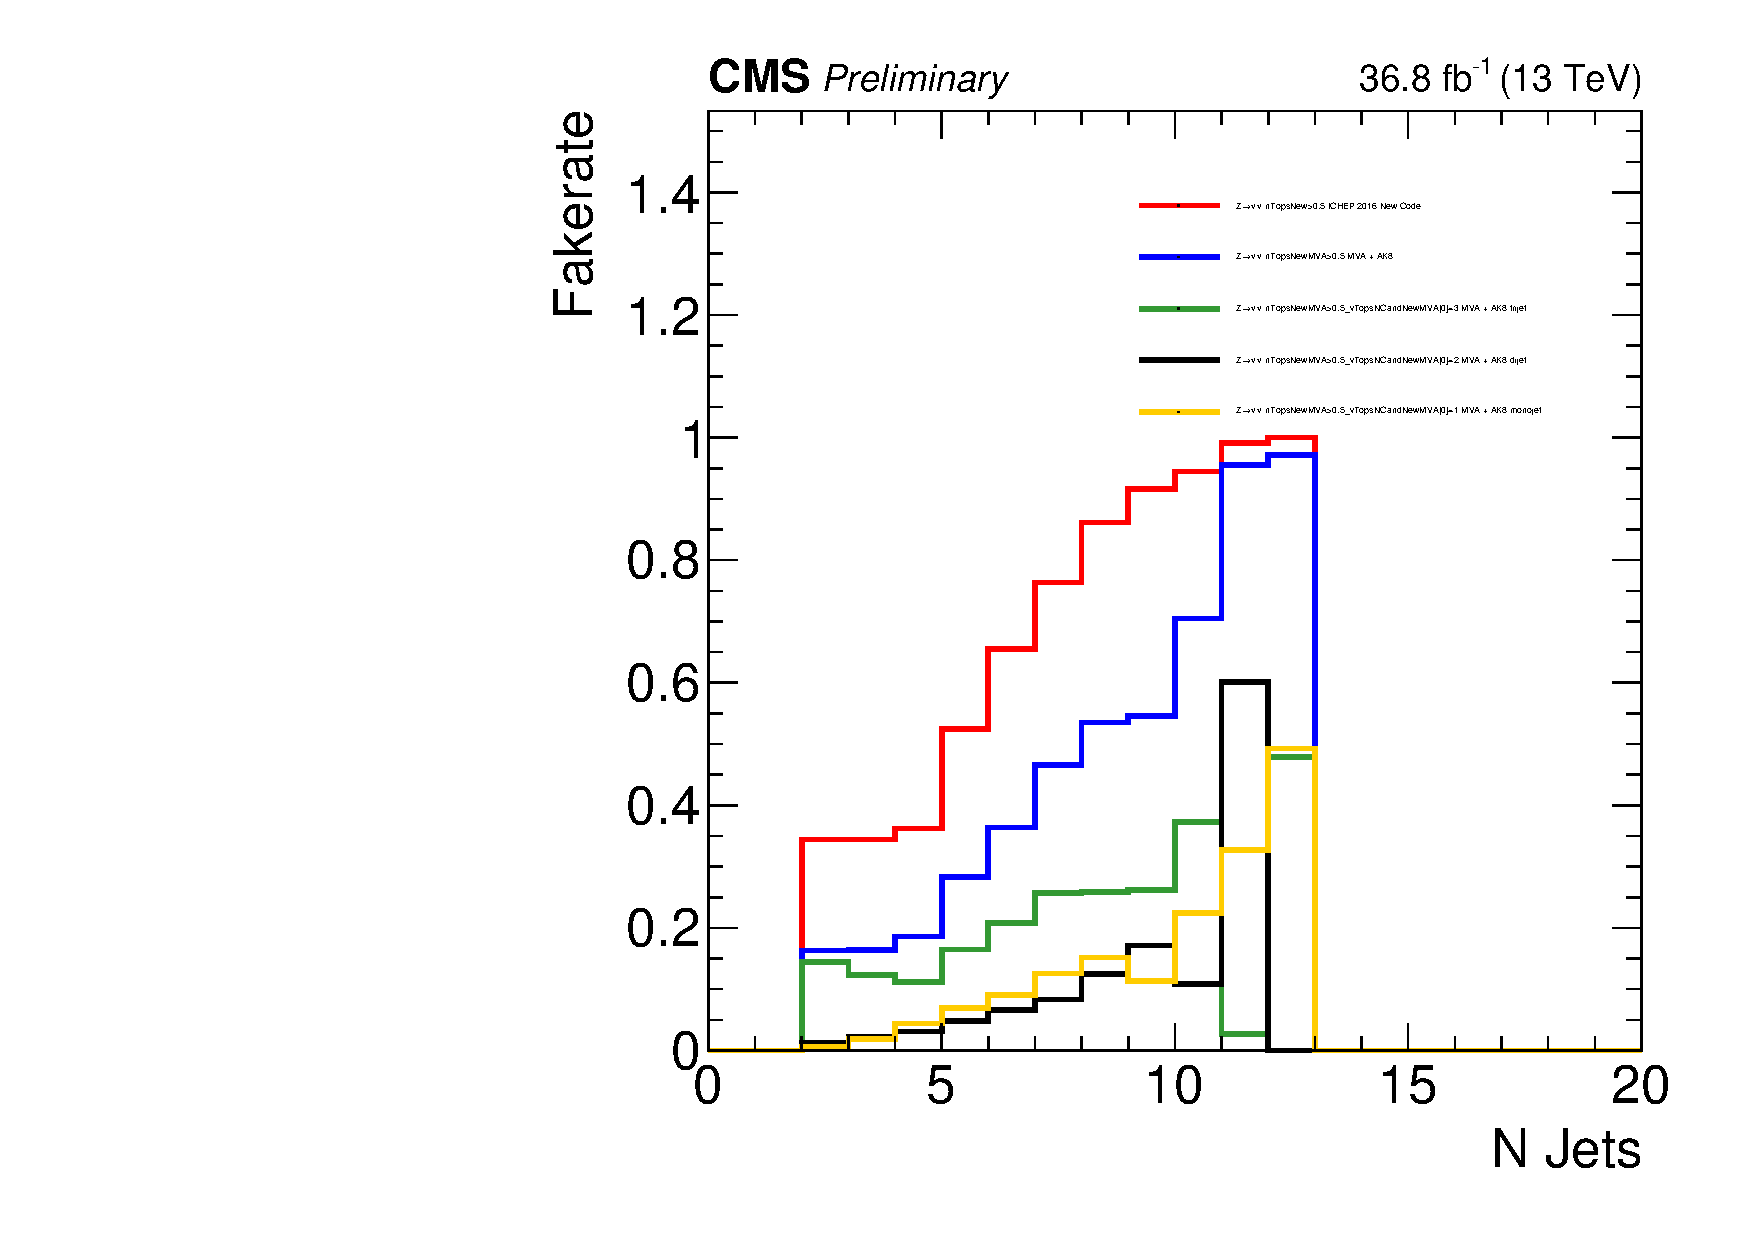
\includegraphics[width=0.45\textwidth]{sections/mc4/TopTagger/figures/baseline_fakerate_njet_tight.pdf}
 \end{center} \caption{Top-jet reconstruction mistag rate, measured in $Z$+jets simulation samples. Left plot is the distribution in \MET, Right plot is in \njets.}
 \label{fig:c4ttmistagtight}
\end{figure}
